\documentclass{report}
\usepackage[utf8]{inputenc}
\usepackage[english]{babel}
\usepackage{amsmath}
\usepackage{amsfonts}
\usepackage{amssymb}
\usepackage{amsthm}
\usepackage[basic]{complexity}
\usepackage{tikz}
\usepackage{hyphenat}
\usepackage{graphicx}
\usepackage{mathpazo}
\usepackage{nicefrac}
\usepackage{fontawesome}
\usepackage{multicol}

\usepackage[authoryear]{natbib}

\usepackage{geometry}
\geometry{vmargin = 2.5cm, hmargin = 2.5cm}

\usepackage{array}
\newcolumntype{L}[1]{>{\raggedright\let\newline\\\arraybackslash\hspace{0pt}}m{#1}}
\newcolumntype{C}[1]{>{\centering\let\newline\\\arraybackslash\hspace{0pt}}m{#1}}
\newcolumntype{R}[1]{>{\raggedleft\let\newline\\\arraybackslash\hspace{0pt}}m{#1}}

\renewcommand{\arraystretch}{1.15}

\usepackage{tikz}
\usetikzlibrary{automata, positioning, calc, shapes, arrows, fit}
\newcommand{\circled}[1]{\tikz[baseline=(char.base)]{
		\node[shape=circle, draw, inner sep=0.5pt] (char) {#1};}}

\usepackage[unicode=true, bookmarks=false, breaklinks=true, pdfborder={0 0 1},colorlinks=true]{hyperref}
\hypersetup{linkcolor=blue,citecolor=blue,filecolor=blue,urlcolor=blue}


\begin{document}
	\title{Preflib 2.0}
	\author{Simon Rey, Nick Mattei}
	\maketitle
	
	\tableofcontents
	
	\chapter{Developing PrefLib}
	
	In this chapter, we detail the inner structure of PrefLib. We will first focus on the folder structure, explaining the role of each file. The second part of this chapter is devoted to the structure of the database. 
	
	The aim of this chapter is to provide all the necessary information to someone who would like to develop further the website. If you are only interested in maintaining the website and do some small changes, the second chapter might be more interesting to you.
	
	\section{Folder Structure}
	
	The folder structure of the project follows that of a typical Django project with one application. The overall Django project is called \texttt{preflib} and the main, and only, django application is called \texttt{preflibApp}. The overall folder structure can be found in Figure \ref{fig:folderStruct}. In what follows, we give an explanation for each folder and files.
	
	\begin{figure}
		\begin{multicols}{2}
			\begin{itemize}
				\item[\faFolderO] preflib
				\begin{itemize}
					\item[\faFileO] settings.py
					\item[\faFileO] urls.py
					\item[\faFileO] wsgi.py
				\end{itemize}
				\item[\faFolderO] preflibApp
				\begin{itemize}
					\item [\faFolderO] management
					\begin{itemize}
						\item[\faFolderO] commands
						\begin{itemize}
							\item[\faFileO] adddataset.py
							\item[\faFileO] generatezip.py
							\item[\faFileO] initializedb.py
							\item[\faFileO] updatemetadata.py
							\item[\faFileO] updatepapers.py
						\end{itemize}
					\end{itemize}
					\item[\faFolderO] preflibtools
					\begin{itemize}
						\item[\faFileO] drawing.py
						\item[\faFileO] graph.py
						\item[\faFileO] instance.py
						\item[\faFileO] properties.py
					\end{itemize}
					\item[\faFolderO] static
					\begin{itemize}
						\item[\faFolderO] adminLogo
						\begin{itemize}
							\item[\faFilesO] images for the admin menu
						\end{itemize}
						\item[\faFolderO] css
						\begin{itemize}
							\item[\faFileO] nouislider.css
							\item[\faFileO] style.css
						\end{itemize}
						\item[\faFolderO] data
						\begin{itemize}
							\item[\faFolderO] CD
							\item[\faFolderO] ED
							\item[\faFolderO] MD
							\item[\faFolderO] types
						\end{itemize}
						\item[\faFolderO] datatoadd
						\item[\faFolderO] js 
						\begin{itemize}
							\item[\faFileO] nouislider.js
						\end{itemize}
						\item[\faFolderO] types
						\begin{itemize}
							\item[\faFileO] dataTypesImages.tex
							\item[\faFilesO] images to present the types
						\end{itemize}
						\item[\faFileO] crisner.png
						\item[\faFileO] gitHubLogo.png
						\item[\faFileO] papers.bib
						\item[\faFileO] preflibADTCite.txt
						\item[\faFileO] preflibADTPaper.pdf
						\item[\faFileO] preflibTrendsComSoCChapter.pdf
						\item[\faFileO] preflibTrendsComSoCCite.txt
					\end{itemize}
					\item[\faFolderO] templates
					\begin{itemize}
						\item[\faFolderO] includes
						\begin{itemize}
							\item[\faFilesO] HTML files that can be included
						\end{itemize}
						\item[\faFolderO] preflib
						\begin{itemize}
							\item[\faFilesO] main HTML files
						\end{itemize}
						\item[\faFileO] 400.html
						\item[\faFileO] 403.html
						\item[\faFileO] 404.html
						\item[\faFileO] 500.html
					\end{itemize}
					\item[\faFolderO] templatetags
					\begin{itemize}
						\item[\faFileO] extratags.py
					\end{itemize}
					\item[\faFileO] admin.py
					\item[\faFileO] apps.py
					\item[\faFileO] choices.py
					\item[\faFileO] forms.py
					\item[\faFileO] models.py
					\item[\faFileO] scripts.py
					\item[\faFileO] urls.py
					\item[\faFileO] views.py
				\end{itemize}
			\end{itemize}
		\end{multicols}
		\caption{Folder Structure of the Project, some less relevant files have been omitted.}
		\label{fig:folderStruct}
	\end{figure}

	\subsection*{\faFolderO{}  preflib}
	
	The \texttt{preflib} folder contains the files that have an impact on the entire project. This is the highest folder in the Django hierarchy. Files in there are mainly used to set up the global parameters of the project.
	
	\paragraph*{\faFileO{} settings.py} This is the main files for the global settings. Among other things, you will find there the settings for the database, the location of the static files, the debugging mode, the installed applications, ... Not that this file is not on the git for security reasons.
	
	\paragraph*{\faFileO{} urls.py} Use this file to set up the global rules for urls. Whenever a request passed over to Django, this file is used to decide where to send the request next. Handlers for the errors (404, 500, etc...) are also defined there.
	
	\paragraph*{\faFileO{} wsgi.py} This is only used to set up the connection between Django and whatever WSGI tool is used (uWSGI, Gunicorn, Passenger). If you did not understand the previous sentence, you will most likely never have to deal with this file.
	
	\subsection*{\faFolderO{} preflibApp/management/commands}
	
	The \texttt{management/commands} folder includes the user-defined commands that one can access using the Django's management tool. Each file in this folder contains a class \texttt{Command} which should contain some specific methods. Importantly, once defined and put in this folder, the command can be accessed as any other management command, for instance from the command line using: \texttt{python3 manage.py adddataset}.
	
	\paragraph*{\faFileO{} adddataset.py} This command is used to add datasets to the database. Only zip files located in the folder \texttt{static/datatoadd} can be retrieved by this command. Two arguments can be passed to the command, either \texttt{--file zipfilename} to add only a specific zip file, or \texttt{--all} to add all the zip files in the \texttt{static/datatoadd} folder to the database.
	
	When adding a dataset, the command unzip the archive in a temporary folder. It then goes through the files to find the info file used to get all the information for the dataset. Then, each file is added to the database, together with its datapatch (if needed). Note that the metadata are not computed when adding a dataset. 
	
	\paragraph*{\faFileO{} generatezip.py} This command is used to generate all the zip files served by the website. It first generates the zip files for the dataset, creating the info file with the entry in the database. In a second time, it generates the zip files per type of data.
	
	\paragraph*{\faFileO{} initializedb.py} This command is only run once, at the very beginning, to populate the database with the entries that are needed. It mainly sets up the metadata.
	
	\paragraph*{\faFileO{} updatemetada.py} This command computes the metadata for the data files. Two options can be passed to the command. When used with \texttt{--dataset datasetAbbreviation}, only the metadata for the given dataset will be computed. One can also use \texttt{--noDrawing} to avoid generating the images for the data file (which takes a lot of time).
	
	For each relevant data file, the command will go through all the \emph{active} metadata (see later what active mean here). Whenever an active metadata applies to the data type of the data file, the corresponding function is called to compute its value. If drawing is allowed, the relevant drawing method is also called.
	
	\paragraph*{\faFileO{} updatepapers.py} This command updates the list of papers that are using Preflib. It reads the bib file \texttt{static/papers.bib} and update the database accordingly.
	
	\subsection*{\faFolderO{} preflibApp/preflibtools} This folder contains the tools that were developed around PrefLib to work with the data. Note that this version is far from what you can find in the PrefLibTools repository on GitHub. These tools are mainly used to analyze the data when computing the relevant metadata.
	
	\paragraph*{\faFileO{} drawing.py} This file contains all the functions that are used to draw the images representing the data. 
	
	\paragraph*{\faFileO{} graph.py} This file contains the definition of the \texttt{Graph} class that we use to represent graphs and access several useful methods for them.
	
	\paragraph*{\faFileO{} instance.py} This file contains the class used to represent PrefLib instances. The methods for parsing the data file are defined there.
	
	\paragraph*{\faFileO{} properties.py} This file contains a collection of functions used to check whether some properties hold for a given instance. This is the main file used to compute the metadata of the instances.
	
	\subsection*{\faFolderO{} preflibApp/static}
	
	The \texttt{static} folder contains all the static files that are used (unsurprisingly). This folder is the one considered by the \texttt{collecstatic} management command from Django.
	
	\paragraph*{\faFolderO{} adminLogo} The folder gathers all the images of the logo used for the admin menu. Note that it might disappear in some later versions.
	
	\paragraph*{\faFolderO{} css}
	
	\paragraph*{\faFolderO{} js}
	
	\paragraph*{\faFolderO{} types}
	
	\paragraph*{\faFileO{} crisner.png}
	
	\paragraph*{\faFileO{} gitHubLogo.png}
	
	\paragraph*{\faFileO{} papers.bib}
	
	\paragraph*{\faFilesO{} preflib citations}
	
	
	\subsection*{\faFolderO{} preflibApp/templates}
	
	\subsection*{\faFolderO{} preflibApp/templatetags}
	
	\subsection*{\faFolderO{} preflibApp}
		
	\begin{itemize}
		\item preflib
		\begin{itemize}
			\item settings.py: all the inner settings of the project, only change things there if you know what you're doing.
			\item urls.py: general patterns for URL, since there only is one application the file is quite basic. Handlers for errors (500, 404, ...) also are defined there.
			\item wsgi.py: used to link django to the http server, do not modify.
		\end{itemize}
		\item preflibApp
		\begin{itemize}
			\item management/commands
			\begin{itemize}
				\item adddataset.py: management command used to add a dataset to the database.
				\item createmetadata.py: command to generate all the metadata for the datafile in the database.
				\item generatezip.py: generates all the zip files.
				\item initializedb.py: command to be run when setting up the website.
				\item updatepapers.py: update the list of the papers using Preflib according the a bib file.
			\end{itemize}
			\item migrations: inner Django stuff, do not modify.
			\item preflibtools: nothing to do with Django, all the tools used to deal with the data.
			\item static: all the static files that are served by the website.
			\item templates: a template is an html file which can incorporate some Django code to perform some computations in it. This folder contains the general html structure of the website, i.e., all its templates.
			\item templatetags: custom tags that can be used in the templates.
			\item admin.py: define which tables can be accessed on the Django admin page of the website.
			\item apps.py: inner Django stuff, do not modify.
			\item choices.py: several fields in the database have to be selected among a specific list. All the lists that are not worth putting in the database (because they never change for instance) are defined here.
			\item forms.py: the Django representation of the html forms that are used in the website. It is for instance, the login form, some administrative forms...
			\item models.py: all Danjgo objects representing the tables in the database. This is an important file that describes the entire database structure.
			\item scripts.py: some useful scripts, mainly used for management purposes.
			\item urls.py: the URL pattern for the pages available through this app.
			\item views.py: the most important file. The views are functions that are called to render the page requested by the user. This is where all the computations that are done at runtime are described.
		\end{itemize}
		\item manage.py: Python file to run local functions
	\end{itemize}
	
	\section{Database Structure}
	
	In the following, we provide more details about the structure of the database behind Preflib.
	
	\medskip
	
	Let us first go through all the tables present in the database.
	
	\paragraph{\textsc{DataFile}} The most fundamental entity for Preflib is the datafile. The \textsc{DataFile} table contains a reference to all the datafiles that are in Preflib. The table does not contain the data in itself---it is stored in a file and not in the database---but all the relevant information about it: some basic details and datapatch in which the file is.
	
	\paragraph{\textsc{DataPatch}} The datapatch is the first level of classification of the datafile. It contains several datafile of different datatype. All the datafiles are based on the same preferences but the representation, the datatype, is different.
	
	\paragraph{\textsc{DataSet}} A dataset is a collection of datapatches. The datapatches will typically represent different years of the same election.
	
	\paragraph{\textsc{DataProperty}} A dataproperty is an additional information about a given datafile. It can have to do about the general properties of the data (number of candidates...) or about some more specific structure of the data (single-peakedness...).
	
	\paragraph{\textsc{Metadata}} The \textsc{Metadata} table stores all the different metadata available in the system. Their values are in the \textsc{DataProperty} table.
	
	\paragraph{\textsc{Paper}} This table stores the information about the papers which are using Preflib.
	
	\paragraph{\textsc{UserProfile}} All the informations about the users that are not in the Django User class are present in this table.
	
	\paragraph{\textsc{Log}} Logs of what is happening in the inside are gathers in this table.
	
	\medskip
	
	The following figure summarizes the links between the different tables and presents all the elements present in the tables.
	
	\begin{center}
		\resizebox{\linewidth}{!}{
		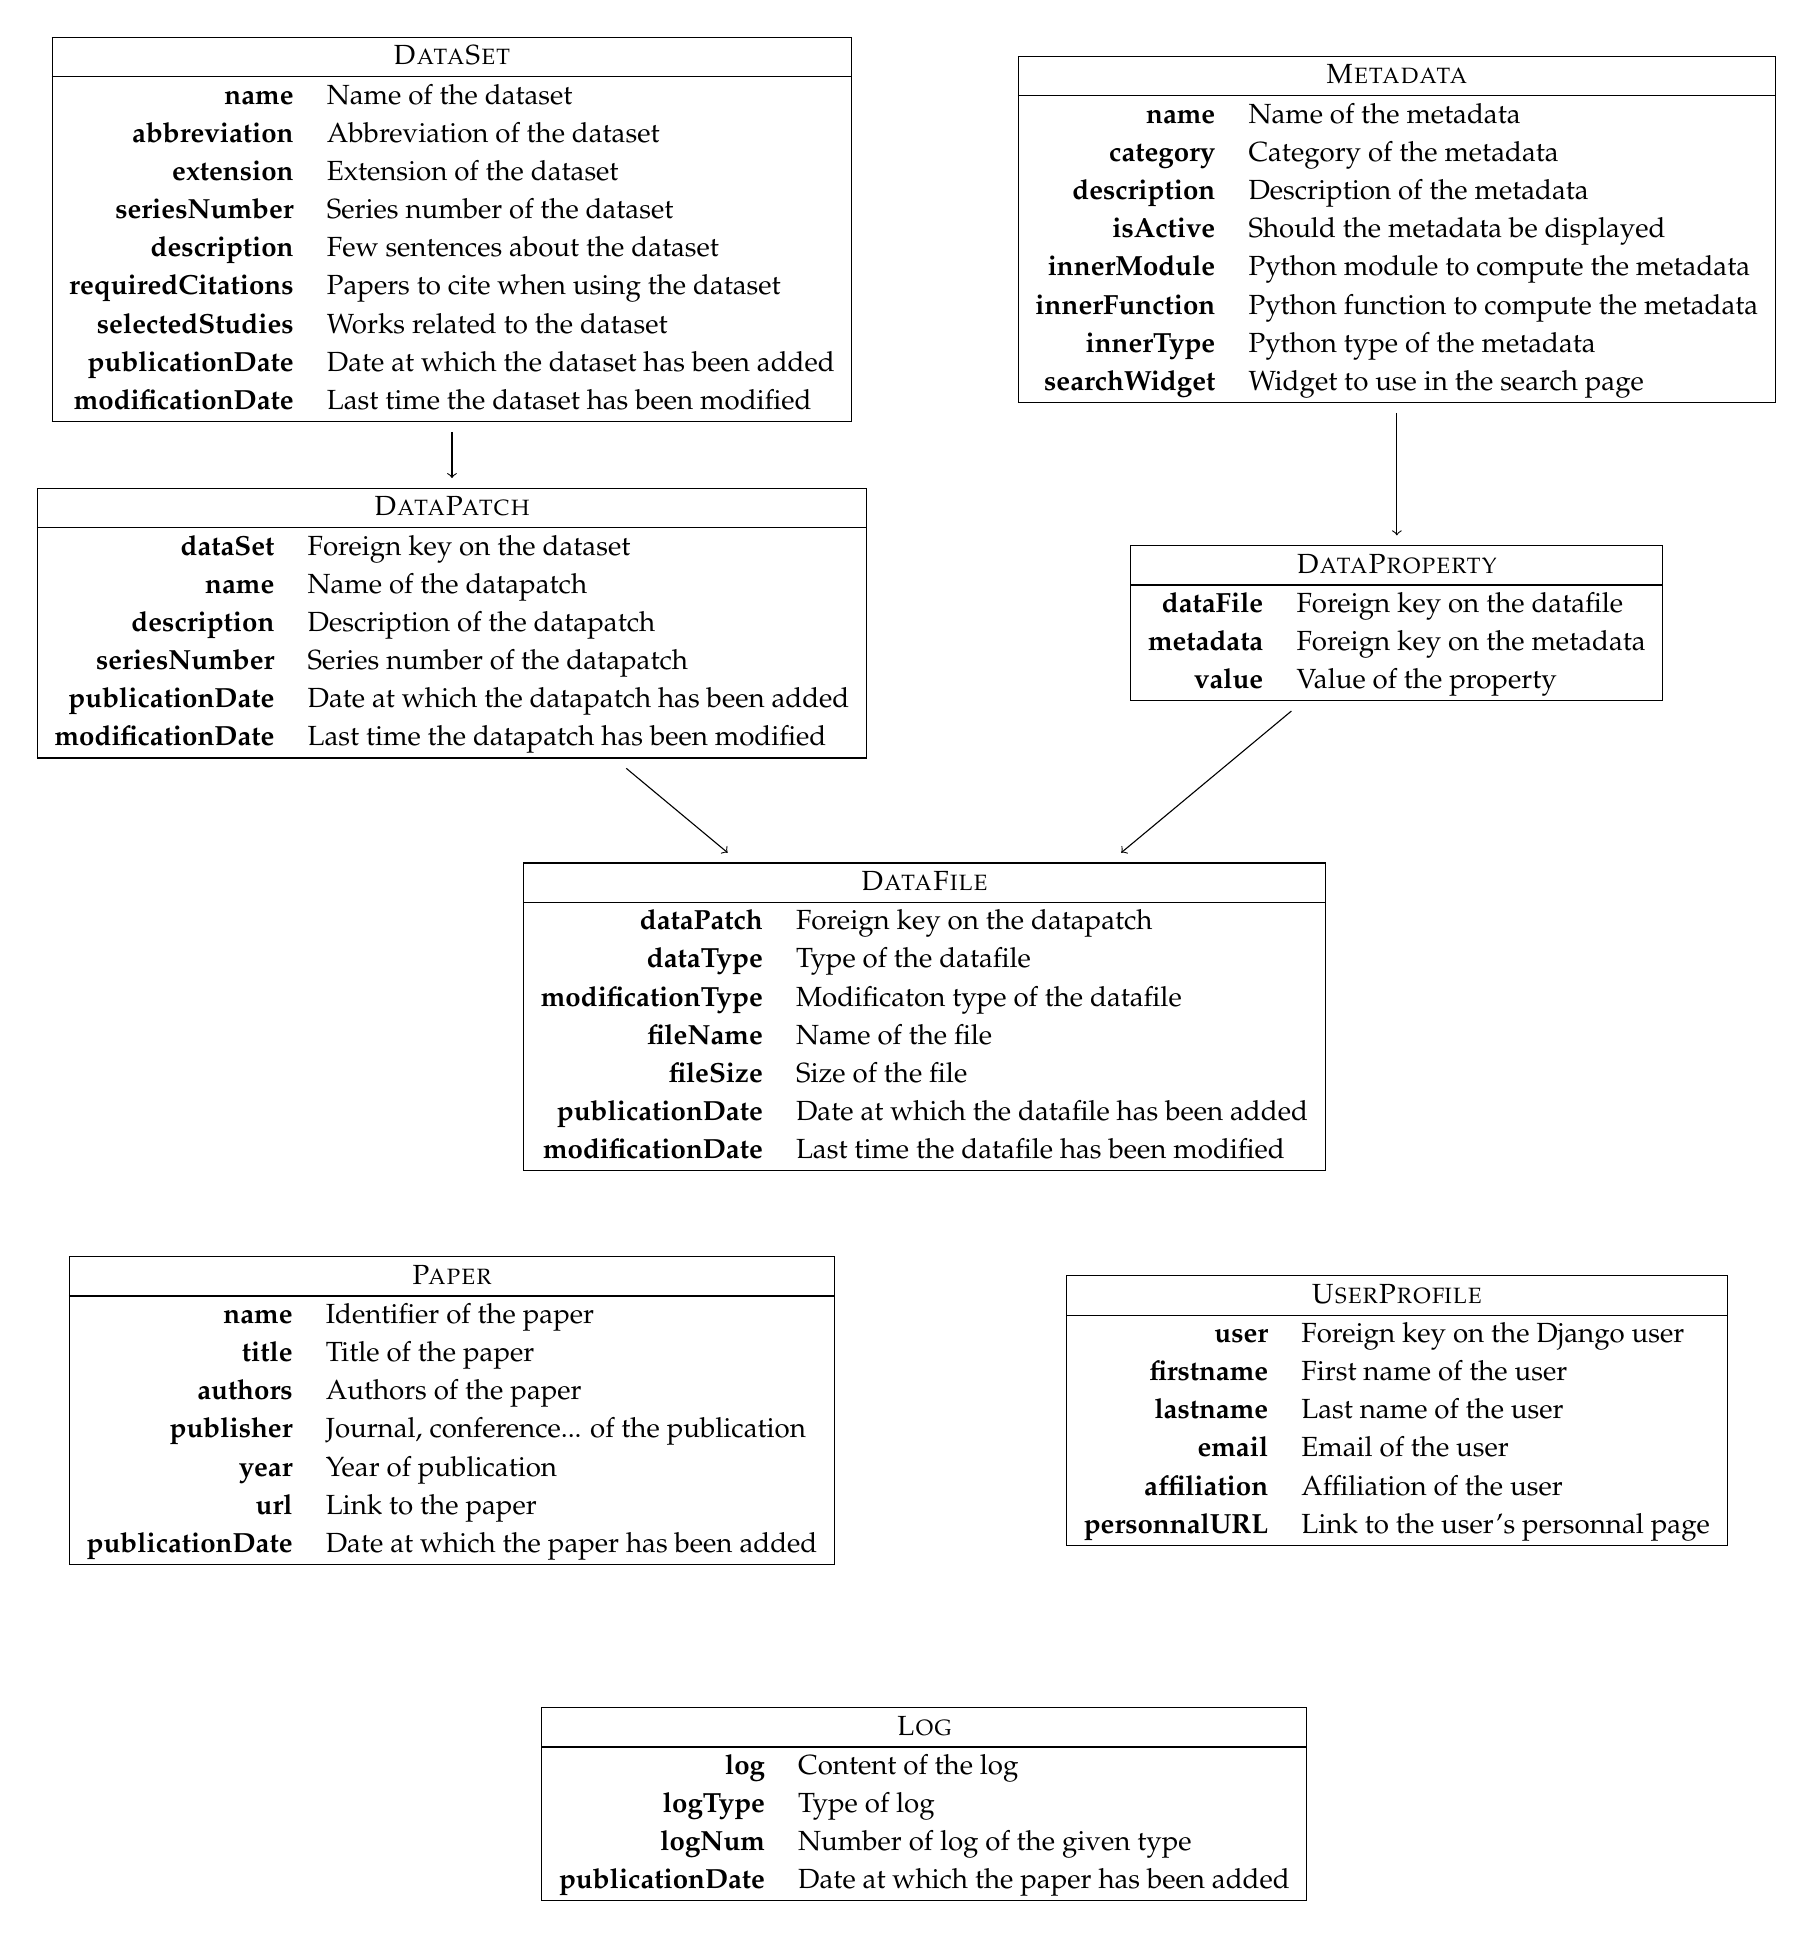
\begin{tikzpicture}
			\node[] (dataset) at (0, 0) {\begin{tabular}{|rl|}
					\hline
					\multicolumn{2}{|c|}{\textsc{DataSet}} \\
					\hline
					\textbf{name} & Name of the dataset \\
					\textbf{abbreviation} & Abbreviation of the dataset\\
					\textbf{extension} & Extension of the dataset \\
					\textbf{seriesNumber} & Series number of the dataset\\
					\textbf{description} & Few sentences about the dataset \\
					\textbf{requiredCitations} & Papers to cite when using the dataset \\
					\textbf{selectedStudies} & Works related to the dataset \\
					\textbf{publicationDate} & Date at which the dataset has been added \\
					\textbf{modificationDate} & Last time the dataset has been modified \\
					\hline
			\end{tabular}};
			
			\node[] (datapatch) at (0, -5) {\begin{tabular}{|rl|}
					\hline
					\multicolumn{2}{|c|}{\textsc{DataPatch}} \\
					\hline
					\textbf{dataSet} & Foreign key on the dataset \\
					\textbf{name} & Name of the datapatch \\
					\textbf{description} & Description of the datapatch \\
					\textbf{seriesNumber} & Series number of the datapatch \\
					\textbf{publicationDate} & Date at which the datapatch has been added \\
					\textbf{modificationDate} & Last time the datapatch has been modified\\
					\hline
			\end{tabular}};
			
			\node[] at (6, -10) (datafile) {\begin{tabular}{|rl|}
					\hline
					\multicolumn{2}{|c|}{\textsc{DataFile}} \\
					\hline
					\textbf{dataPatch} & Foreign key on the datapatch \\
					\textbf{dataType} & Type of the datafile\\
					\textbf{modificationType} & Modificaton type of the datafile\\
					\textbf{fileName} & Name of the file  \\
					\textbf{fileSize} & Size of the file \\
					\textbf{publicationDate} & Date at which the datafile has been added \\
					\textbf{modificationDate} & Last time the datafile has been modified\\
					\hline
			\end{tabular}};
		
			\node[] (metadata) at (12, 0) {\begin{tabular}{|rl|}
					\hline
					\multicolumn{2}{|c|}{\textsc{Metadata}} \\
					\hline
					\textbf{name} & Name of the metadata \\
					\textbf{category} & Category of the metadata \\
					\textbf{description} & Description of the metadata \\
					\textbf{isActive} & Should the metadata be displayed \\
					\textbf{innerModule} & Python module to compute the metadata \\
					\textbf{innerFunction} &  Python function to compute the metadata \\
					\textbf{innerType} & Python type of the metadata \\
					\textbf{searchWidget} & Widget to use in the search page\\
					\hline
			\end{tabular}};
			
			\node[] (dataprop) at (12, -5) {
				\begin{tabular}{|rl|}
					\hline
					\multicolumn{2}{|c|}{\textsc{DataProperty}} \\
					\hline
					\textbf{dataFile} & Foreign key on the datafile \\
					\textbf{metadata} & Foreign key on the metadata \\
					\textbf{value} & Value of the property \\
					\hline
			\end{tabular}};
		
			\draw[->] (dataset) edge (datapatch);
			\draw[->] (datapatch) edge (datafile);
			\draw[->] (metadata) edge (dataprop);
			\draw[->] (dataprop) edge (datafile);
			
			\node[] (paper) at (0, -15) {\begin{tabular}{|rl|}
					\hline
					\multicolumn{2}{|c|}{\textsc{Paper}} \\
					\hline
					\textbf{name} & Identifier of the paper \\
					\textbf{title} & Title of the paper \\
					\textbf{authors} & Authors of the paper \\
					\textbf{publisher} & Journal, conference... of the publication \\
					\textbf{year} & Year of publication \\
					\textbf{url} &  Link to the paper \\
					\textbf{publicationDate} & Date at which the paper has been added \\
					\hline
			\end{tabular}};
		
			\node[] (userprofile) at (12, -15) {\begin{tabular}{|rl|}
					\hline
					\multicolumn{2}{|c|}{\textsc{UserProfile}} \\
					\hline
					\textbf{user} & Foreign key on the Django user \\
					\textbf{firstname} & First name of the user \\
					\textbf{lastname} & Last name of the user \\
					\textbf{email} & Email of the user \\
					\textbf{affiliation} & Affiliation of the user \\
					\textbf{personnalURL} &  Link to the user's personnal page \\
					\hline
			\end{tabular}};
			
			\node[] (Log) at (6, -20) {\begin{tabular}{|rl|}
					\hline
					\multicolumn{2}{|c|}{\textsc{Log}} \\
					\hline
					\textbf{log} & Content of the log \\
					\textbf{logType} & Type of log \\
					\textbf{logNum} & Number of log of the given type \\
					\textbf{publicationDate} & Date at which the paper has been added \\
					\hline
			\end{tabular}};
		\end{tikzpicture}}
	\end{center}

	\chapter{Maintaining PrefLib}
	
\end{document}